\documentclass[]{paper}
\usepackage{graphicx}
\usepackage{color}

% type user-defined commands here
\newif\ifdraft
\drafttrue
\ifdraft
\newcommand{\onote}[1]{ {\textcolor{cyan} { (***Ole: #1) }}}
\newcommand{\terminology}[1]{ {\textcolor{red} {(Terminology used: \textbf{#1}) }}}
\newcommand{\owave}[1]{ {\cyanuwave{#1}}}
\newcommand{\jwave}[1]{ {\reduwave{#1}}}
\newcommand{\alwave}[1]{ {\blueuwave{#1}}}
\newcommand{\jhanote}[1]{ {\textcolor{red} { ***shantenu: #1 }}}
\newcommand{\alnote}[1]{ {\textcolor{green} { ***andreL: #1 }}}
\newcommand{\amnote}[1]{ {\textcolor{blue} { ***andreM: #1 }}}
\newcommand{\smnote}[1]{ {\textcolor{brown} { ***sharath: #1 }}}
\newcommand{\pmnote}[1]{ {\textcolor{brown} { ***Pradeep: #1 }}}
\newcommand{\msnote}[1]{ {\textcolor{cyan} { ***mark: #1 }}}
\newcommand{\note}[1]{ {\textcolor{magenta} { ***Note: #1 }}}
\else
\newcommand{\onote}[1]{}
\newcommand{\terminology}[1]{}
\newcommand{\owave}[1]{#1}
\newcommand{\jwave}[1]{#1}
\newcommand{\alnote}[1]{}
\newcommand{\amnote}[1]{}
\newcommand{\athotanote}[1]{}
\newcommand{\smnote}[1]{}
\newcommand{\pmnote}[1]{}
\newcommand{\jhanote}[1]{}
\newcommand{\msnote}[1]{}
\newcommand{\note}[1]{}
\fi

\begin{document}

\title{FutureGrid 2012 Project Challenge: Interoperable and
  Standards-based Distributed Cyberinfrastructure and Applications}
 
\author{Andre Luckow 
  \and Andre Merzky
  \and Mark Santcroos
  \and Ole Weidner 
  \and Shantenu Jha
}
\date{May 15th, 2012}
\maketitle

\begin{abstract}
\end{abstract}

\section{Introduction}

FutureGrid provides researchers with new possibilities to engage in
science relating to the state-of-the-art in cloud and grid
computing. As members of the RADICAL group, we have taken full
advantage of the opportunities that FutureGrid provides. Here are some
of the ways we are using FutureGrid resources to push the envelope and
pursue exciting new discoveries.

\jhanote{Topics to be covered: (i) P* (AL) (ii) CSA ? (AM) (iii)
  OGF-Standards based development and testing (AM) (iv) Class Project
  (SJ) (v) Others?}

\section{P* - Pilot-Job Interoperability}

Pilot-Jobs (PJ) have become one of the most successful abstractions in
distributed computing. In spite of extensive uptake, there does not exist a
well defined, unifying conceptual model of Pilot-Jobs, which can be used to
define, compare and contrast PJ implementations. This presents a barrier to
extensibility and interoperability. The P*
model~\cite{pstar-2012,pstar-sc-2012} provide a minimal but complete model of
Pilot-Jobs, which has been successfully applied to different Pilot-Job
frameworks, e.\,g.\ Condor and DIANE. The Pilot-API~\cite{pilot_api} provides 
an abstract, unified interface to PJ frameworks that adhere to the P* Model.

To demonstrated the interoperable and concurrent use of multiple Pilot-Job
frameworks via the Pilot-API on different production and research
infrastructures. Figure~\ref{fig:perf_perf-bfast-bj} shows how the Pilot-API
enables the user to run applications interoperably on different production and
research infrastructures. For this purpose we investigate the performance of
BFAST, a genome sequencing application. BFAST is very I/O sensitive -- we
observed for example, an I/O bottleneck if many BFAST CUs are run on the same
shared file system. The Pilot-API enables applications to scale to different
infrastructures in such cases.

\begin{figure}[t]
\centering
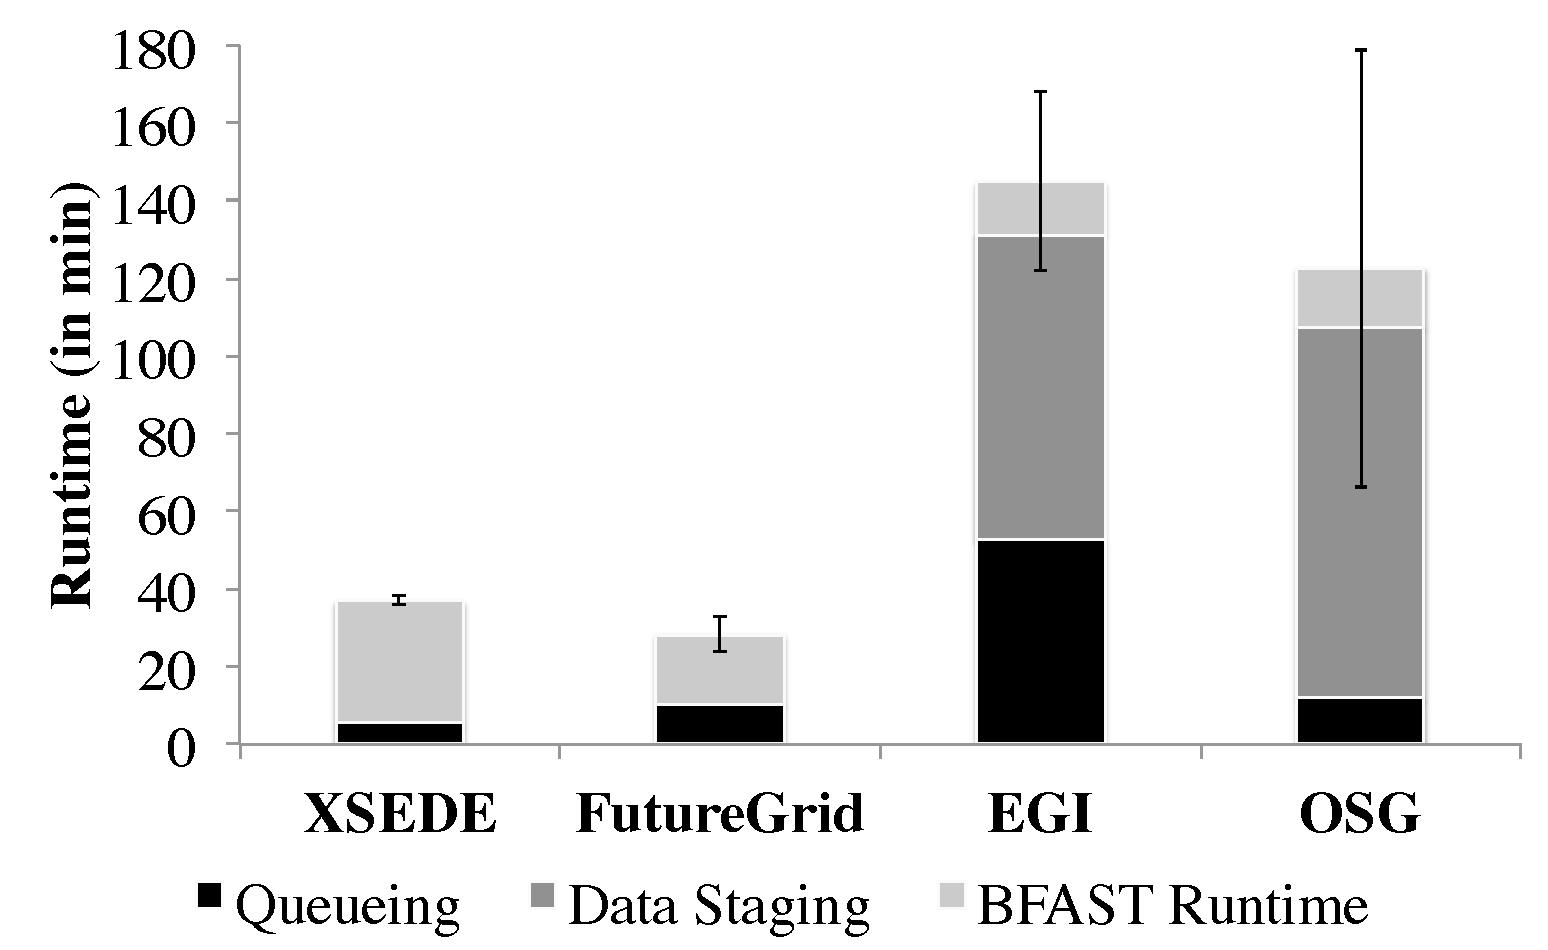
\includegraphics[width=0.7\textwidth]{figures/128-bfast-egi-fg-xsede-osg.pdf}
\caption{\textbf{PJ Framework Performance on XSEDE, FutureGrid, EGI and 
  OSG:} Running 128 BFAST match tasks on 128 cores. The longer runtimes on EGI 
  and OSG are mainly caused by  longer queuing times and the necessity to      
  stage all input files.}
  \label{fig:perf_perf-bfast-bj}
\end{figure}

\section{BigJob and BigData}

FutureGrid has been an important testbed for the development of
BigJob~\cite{saga_bigjob_condor_cloud} and
BigData~\cite{pstar-sc-2012,pmr-2012}. BigJob (BJ) is a SAGA-based Pilot-Job
(PJ) framework that implements the Pilot-API. BJ has been designed to be
general-purpose and extensible. While BJ has been originally built for HPC
infrastructures, such as FutureGrid and XSEDE, it is generally also usable in
other environments, such as OSG. This extensibility mainly arises from the
usage of SAGA as a common API for accessing distributed resources.

\begin{figure}[t]
	\centering
	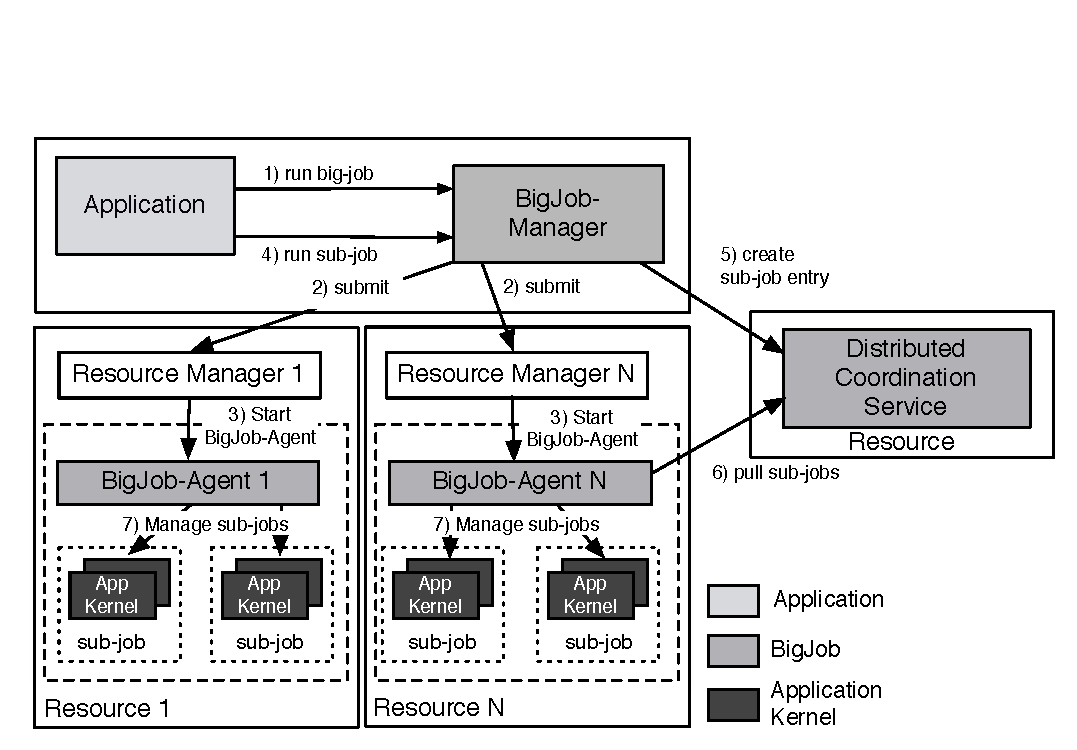
\includegraphics[width=0.7\textwidth]{figures/re_bigjob_interactions.pdf}
	\caption{\textbf{BigJob Architecture:} The
	          BJ architecture resembles many elements of the P* Model. The
	          BigJob-Manager is the central Pilot-Manager, which
	          orchestrates a set of Pilots. Each Pilot is represented by a
	          decentral component referred to as the BigJob-Agent.}
			\label{fig:figures_re_bigjob_interactions}
\end{figure}

Figure~\ref{fig:figures_re_bigjob_interactions} illustrates the BJ
architecture: The BJ-Manager is the Pilot-Manager responsible for coordinating
the different components of the frameworks. The BigJob-Agent is the actual
Pilot that is submitted to a resource. BigData extends the Pilot-Job concept
to data. BigData provides late-binding capabilities for data by separating the
storage allocation and application-level~\cite{pstar-2012}. Similar to BigJob,
it is comprised of two components: the BD-Manager and the BD-Agents, which are
deployed on the physical resources.

\begin{figure}[t] 
\centering 
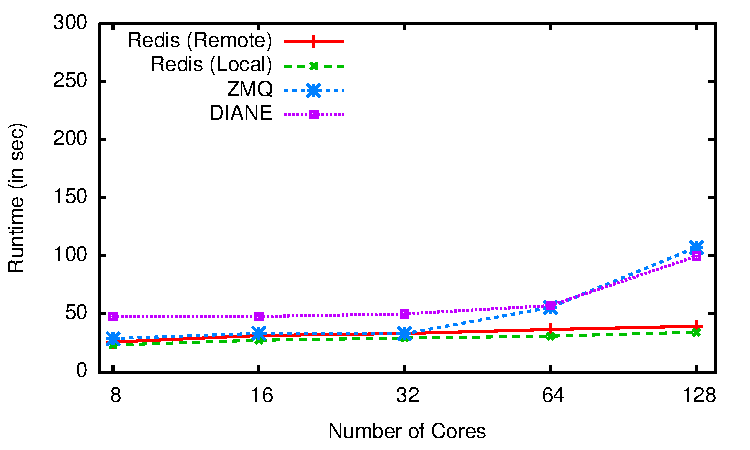
\includegraphics[width=0.8\textwidth]{figures/bigjob-varying-cores-alamo-noadvert.pdf}
\caption{\textbf{Pilot-Job Coordination Mechanism:}  The runtime of a
workload of 4 tasks per core, i.\,e.\ 32 - 512\,tasks, using different Pilots
and configuration. For BJ-Redis the runtime  increases only moderately, the
client-server-based implementations BJ-ZMQ and CORBA-based DIANE show
particularly a steep increase when going from 64 to 128 cores.}
\label{fig:perf_bigjob-varying-cores} 
\end{figure}

We used FutureGrid to evaluate the overheads typical associated with PJ
frameworks. For the evaluation of the communication \& coordination (c\&c)
subsystem of BigJob and DIANE we run a different number of very short running
(i.\,e. zero workload) tasks on Alamo/FG concurrently. In general, the c\&c
systems used are mostly insensitive to the number of coordinated tasks.

Figure~\ref{fig:perf_bigjob-varying-cores} illustrates the scalability of BJ
and DIANE with respect to the number of cores and tasks managed by Pilot. For
this purpose, we execute 4\,tasks per core, i.\,e.\ between 32 and 512\,tasks.
BigJob with Redis (local) shows almost linear scaling up to 128 cores. BigJob
with Redis (remote) imposes an increase of about 14\,\%. BigJob with ZeroMQ
performs very well with lower core counts; with larger core counts, the
runtimes increase, indicating a potential scalability bottleneck. Due to
higher startup overhead, at lower core counts DIANE shows a longer runtime
than ZeroMQ or Redis. At higher core counts DIANE behaves similar to
BigJob/ZeroMQ, but shows a greater increase in the overall runtime. This
increase is likely attributable to the single central manager in DIANE's
CORBA-based client-server architecture. Using Redis as central data space for
BigJob decouples Pilot-Manager and Agent, yielding better performance in
particular with many replicas.



\section{Replica Exchange}

Various applications have been developed using Pilot Abstractions and BigJob.
An important application class are those based on the Replica-Exchange
algorithm. Replica-Exchange (RE) are used to understand physical phenomena –
ranging from protein folding dynamics to binding affinity calculations. RE
methods represent a class of algorithms that involve a large number of
loosely-coupled ensembles. We develop a framework for RE that supports
different replica-pairing and coordination mechanisms, that can utilize a
range of production cyberinfrastructure concurrently. We use this framework to
implement three different formulations of the RE algorithm: the synchronous, 
asynchronous (centralized) and asynchronous (decentralized) formulation.

\alnote{Main issue: In Async-RE paper we only have TG/LONI numbers}
\jhanote{I'm glad for RE to be removed from this paper and left as
  Sai's contribution in the students paper. He has some graphs for
  that too}


\section{Education: Distributed Scientific Computing}

In Fall of 2010 a new class on Scientific Computing was co-introduced
by Prof. Jha (led by Prof. Gabrielle Allen). The Distributed
Scientific Computing component of this class was led and developed by
Jha.  The module (Fig.~\ref{dsc}) covered the theory and practice of
Distributed Scientific Computing, with an emphasis on production-grade
distributed cyberinfrastructure.

There exist a broad range of computational infrastructure with varying
support for application characteristics, usage modes and even access
policies, all of which influence the usefulness of a given
infrastructure for scientific applications.  This module provided
sufficient understanding of production grade distributed
cyberinfrastructure to enable students to discern and determine which
infrastructure would be appropriate and effective for their
applications.

The module began by motivating the role and need for distributed
computing by understanding six rather different distributed
applications -- and analyzing them for the following points: why
distributed, how distributed and the challenges, success and/or issues
in distributing them. Elements of data-intensive computing and the
role of distributed data were also covered.  After establishing the
{\it essential} role of distributed computing in these applications,
as well as understanding the critical role of {\it execution
  environments} for distributed computing, the students were exposed
to a range of production distributed infrastructures and a brief
overview of the design principles, objectives and application
characteristics supported.  Specific examples of production Grids --
high-throughput as well as high-performance were analyzed.

To appreciate the reasons behind the rise of Cloud Computing, the
module provided a basic overview of the important underlying trend in
computing technology and data-intensive computing. This led to the
broader domain of scientific computing as enabled on commercial
infrastructure (Amazon EC2, Azure) as well as other non-commercial
Cloud offerings

%Clouds emerging infrastructure (eg Amazon EC2, Azure).  
 
Practically, the students were given hands on experience with both
virtualized resource and ``bare-metal'' resources thanks to the
FutureGrid. Students mostly experimented with Eucalyptus on India and
Sierra resources of the FutureGrid, as well as worked with a
SAGA-enabled version of MapReduce.

\begin{figure}[ht]
\centerline{
{\small
\begin{tabular}{|p{0.5cm}|p{3.5cm}|p{11.2cm}|}
\hline
& Lecture & Learning Objectives \\
\hline \hline
  E1 & Introduction to the Practise of Distributed Computing - I& WLCG as a motivating example (order of
  magnitude estimates of number of jobs submitted, data transferred,
  CPU cycles consumed), Distributed Application Exemplars, Analyzing
  why and how distributed, and challenges \& success in distribution.
   Introduction to SAGA and FutureGrid (FG). \\
  \hline
  E2 & Introduction to the Practise of Distributed Computing - II & Examples of Production Grid
  Infrastructure - HPC vs HTC, Research vs Production, Commercial.  Introduction to SAGA; Writing {\it your} first Dist.\ Application.  \\
  \hline
  E3 & Cloud Computing \& &  Cloud Computing. Convergence of
  multiple trends, Understanding Amazon \\
  & Master-Worker Pattern  & Examples of M-W Pattern: SAGA-based
  MapReduce, Word Count Application and Mandelbrot Set.\\
  \hline
  E4 & To Distributed or not to Distribute? & 
  Case Studies, Observations on Distributed Applications, Development
  Objectives; Projects on FG. \\
  \hline
\end{tabular}
}
}
\caption{\label{dsc} Module curricula for Distributed Scientific Computing} 
\end{figure}

The Sapir-Whorf hypotheis implies that ``language influences the
(habitual) thought''. The implication and analog in scientific
computing is that the infrastructure used shapes the
practise and formulation of research. Conversely, ``for a given
scientific application/research question, which cyberinfrastructure
should I use?''. Lecture E2  provided a brief overview and
understanding of available infrastructures, and E4 covered
the reasons and answers behind which infrastructure would be suitable
for a broad range of applications.


\section{Conclusion}


\bibliographystyle{plain}
\bibliography{pilotjob,saga,saga-related}


\end{document}
